\documentclass[a4paper,12pt]{report}
% Alternative Options:
%	Paper Size: a4paper / a5paper / b5paper / letterpaper / legalpaper / executivepaper
% Duplex: oneside / twoside
% Base Font Size: 10pt / 11pt / 12pt

\usepackage[export]{adjustbox}

\usepackage{geometry}
%% Language %%%%%%%%%%%%%%%%%%%%%%%%%%%%%%%%%%%%%%%%%%%%%%%%%
%\usepackage[USenglish]{babel} %francais, polish, spanish, ...
\usepackage[francais]{babel}
\usepackage[T1]{fontenc}
\usepackage[utf8]{inputenc}

\usepackage{verbatim}
\usepackage{lmodern} %Type1-font for non-english texts and characters


%% Packages for Graphics & Figures %%%%%%%%%%%%%%%%%%%%%%%%%%
\usepackage{graphicx} %%For loading graphic files
%\usepackage{subfig} %%Subfigures inside a figure
%\usepackage{pst-all} %%PSTricks - not useable with pdfLaTeX

%% Please note:
%% Images can be included using \includegraphics{Dateiname}
%% resp. using the dialog in the Insert menu.
%% 
%% The mode "LaTeX => PDF" allows the following formats:
%%   .jpg  .png  .pdf  .mps
%% 
%% The modes "LaTeX => DVI", "LaTeX => PS" und "LaTeX => PS => PDF"
%% allow the following formats:
%%   .eps  .ps  .bmp  .pict  .pntg


%% Math Packages %%%%%%%%%%%%%%%%%%%%%%%%%%%%%%%%%%%%%%%%%%%%
\usepackage{amsmath}
\usepackage{amsthm}
\usepackage{amsfonts}


%% Line Spacing %%%%%%%%%%%%%%%%%%%%%%%%%%%%%%%%%%%%%%%%%%%%%
\usepackage{setspace}
%\singlespacing        %% 1-spacing (default)
%\onehalfspacing       %% 1,5-spacing
%\doublespacing        %% 2-spacing
\usepackage{listings}
\lstset{language=C} 
\usepackage{color}

\definecolor{mygreen}{rgb}{0,0.6,0}
\definecolor{mygray}{rgb}{0.5,0.5,0.5}
\definecolor{mymauve}{rgb}{0.58,0,0.82}

\lstset{ %
  backgroundcolor=\color{white},   % choose the background color; you must add \usepackage{color} or \usepackage{xcolor}
  basicstyle=\footnotesize,        % the size of the fonts that are used for the code
  breakatwhitespace=false,         % sets if automatic breaks should only happen at whitespace
  breaklines=true,                 % sets automatic line breaking
  captionpos=b,                    % sets the caption-position to bottom
  commentstyle=\color{mygreen},    % comment style
  deletekeywords={...},            % if you want to delete keywords from the given language
  escapeinside={\%*}{*)},          % if you want to add LaTeX within your code
  extendedchars=true,              % lets you use non-ASCII characters; for 8-bits encodings only, does not work with UTF-8
  frame=single,                    % adds a frame around the code
  keepspaces=true,                 % keeps spaces in text, useful for keeping indentation of code (possibly needs columns=flexible)
  keywordstyle=\color{blue},       % keyword style
  language=C++,                 % the language of the code
  otherkeywords={*,...},            % if you want to add more keywords to the set
  numbers=left,                    % where to put the line-numbers; possible values are (none, left, right)
  numbersep=5pt,                   % how far the line-numbers are from the code
  numberstyle=\tiny\color{mygray}, % the style that is used for the line-numbers
  rulecolor=\color{black},         % if not set, the frame-color may be changed on line-breaks within not-black text (e.g. comments (green here))
  showspaces=false,                % show spaces everywhere adding particular underscores; it overrides 'showstringspaces'
  showstringspaces=false,          % underline spaces within strings only
  showtabs=false,                  % show tabs within strings adding particular underscores
  stepnumber=2,                    % the step between two line-numbers. If it's 1, each line will be numbered
  stringstyle=\color{mymauve},     % string literal style
  tabsize=2,                       % sets default tabsize to 2 spaces
  title=\lstname                   % show the filename of files included with \lstinputlisting; also try caption instead of title
}







%% NOTE POUR CLEMENT : UTILISE LE HEADER CI-DESSUS, IL EST MEILLEUR

%%AJOUTS DE CLEMENT DANS LE HEADER :
\usepackage{fancyhdr}
\pagestyle{fancy}
\lhead{Clément BLANQUET et Rafik CHENNOUF}
\rhead{Page \thepage}
\cfoot{\footnotesize{MI11 - Rapport du TP1 Linux embarqué}}
\renewcommand{\headrulewidth}{0.4pt}
\renewcommand{\footrulewidth}{0.4pt}

\usepackage{titlesec}
\makeatletter
\titleformat{\chapter}[frame]
  {\normalfont}{\filright\enspace \@chapapp~\thechapter\enspace}
  {15pt}{\LARGE\bfseries\filcenter}
\titlespacing*{\chapter}
  {0pt}{0pt}{20pt}
\makeatother

\renewcommand{\thesection}{}
\renewcommand{\thesubsection}{\arabic{section}.\arabic{subsection}}
\makeatletter
\def\@seccntformat#1{\csname #1ignore\expandafter\endcsname\csname the#1\endcsname\quad}
\let\sectionignore\@gobbletwo
\let\latex@numberline\numberline
\def\numberline#1{\if\relax#1\relax\else\latex@numberline{#1}\fi}
\makeatother





\author{Clément BLANQUET et Rafik CHENNOUF}
\title{MI11 - Rapport TP 1 - Linux embarqué}

\begin{document}

\begin{titlepage}

	\centering
	
\includegraphics[width=0.15\textwidth]{sigle_UTC.jpg}\par\vspace{1cm}
	{\scshape\LARGE Université de Technologie de Compiègne \par\vspace{1cm}}	
	{\scshape\Large MI11\par}
	\vspace{1.5cm}
	{\huge\bfseries MI11 - Rapport du TP 1 Linux embarqué\par}
	\vspace{2cm}
	{\Large\itshape Clément BLANQUET et Rafik CHENNOUF\par}
	\vspace{2cm}
	\vfill
% Bottom of the page
	{\large Juin 2017}
\end{titlepage}


\renewcommand{\contentsname}{Sommaire} % Changer le nom de la table des matieres
\tableofcontents
% Les différentes tables
\listoffigures        % Liste des figures




\chapter{Rapport TP 1 - Linux embarqué}

\section{Exercice 1 : Prise en main de la carte DevKit8600}
\subsection{Question 1.1}
La DevKit8600 est basée sur les processeurs AM3359 de Texas Instrument. Elle possède un ARM Cortex-A8 cadencé à 720 MHz avec un boot ROM On-Chip de 176KB. Elle possède un certain nombre d'interfaces comme un port LAN, une entrée/sortie audio, des USB, une interface JTAG... etc.

\subsection{Question 1.2} 
On peut stocker le noyau via TFTP (Trivial File Transfer Protocol) et le système de fichiers via NFS (Network File System).

\subsection{Question 1.3}
Nous avons utilisé une liaison série pour nous connecter avec l'application cutecom.

Voici les paramètres que l'on a utilisés :
\begin{enumerate}
\item Bits per second : 115200
\item Data bits : 8
\item Parity : None
\item Stop bits : 1
\item Flow Control : None
\end{enumerate}

\subsection{Question 1.4}
On constate qu'il y a une erreur au démarrage.

\begin{lstlisting}
TFTP error: 'File not found' (1)

ERROR: can't get kernel image!
\end{lstlisting}

La cible ne peut donc pas démarrer. Le fichier manquant est l'image du kernel, appelé \textbf{uImage}.
Il faudrait la placer dans le dossier /tftpboot sur notre PC, puisque la cible nous indique au démarrage qu'elle va cherche l'image à cet endroit.

\subsection{Question 1.5}
Même si l'image était présente, la cible ne pourrait pas démarrer car il manque un rootfs (système de fichier racine).

\section{Exercice 2}
\subsection{Question 2.1}
Le dossier \textit{/home/mi11/poky/build/conf} contient les fichiers de configurations de poky qui permettent donc de configurer l'image selon nos besoins :
\begin{itemize}
\item bblayers.conf
\item local.conf
\item sanity\_info
\item templateconf.cfg
\end{itemize}

Le dossier \textit{/home/mi11/devkit8600/meta-devkit8600} contient les fichiers spécifiques à notre cible qui vont permettre de construire une image qui lui est adaptée.

\subsection{Question 2.2}
Nous avons ajouté une ligne dans le fichier bblayers.conf :

\begin{lstlisting}
BBLAYERS ?= " \
  /home/mi11/poky-dizzy-12.0.3/meta \
  /home/mi11/poky-dizzy-12.0.3/meta-yocto \
  /home/mi11/poky-dizzy-12.0.3/meta-yocto-bsp \
  /home/mi11/devkit8600/meta-devkit8600 \  // CELLE LA
  "
\end{lstlisting}

De plus, à la ligne 36 du fichier local.conf, nous avons inscrit :

\begin{lstlisting}
MACHINE ??= "devkit8600"
\end{lstlisting}

Le nom "devkit8600" est en fait le nom du fichier de configuration du même nom situé ici : 
\textit{/home/mi11/devkit8600/meta-devkit8600/conf/machine}, ce qui fait donc le lien entre la génération de l'image et les paramètres de la cible.

\subsection{Question 2.3}
Voici ce qu'on obtient dans le dossier \textit{/home/mi11/poky/build/tmp/deploy/images} après la compilation : \smallbreak

\begin{figure}
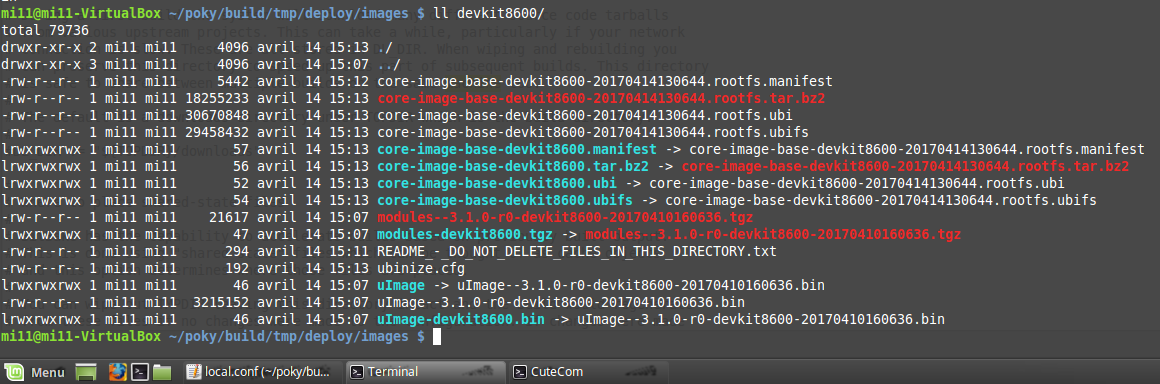
\includegraphics[width=1\textwidth]{23dossierimage.PNG}
\caption{Dossier image} \bigbreak
\end{figure}


On obtient notre image kernel \textit{uImage} qui est en fait un lien symbolique vers le fichier \textit{uImage--3.1.0-r0-devkit8600-20170410160636.bin}.

On voit également le système de fichier nommé \textit{rootfs} qui est compressé dans une archive bzip2.

Si on compare la taille des fichiers qui viennent d'être générés avec ceux de notre VM sous Linux Mint :

\begin{itemize}
\item CIBLE :
\begin{itemize}
\item Taille image : 3,2 MB
\item Taille rootfs : 1,8 MB
\end{itemize}
\item HOTE :
\begin{itemize}
\item Taille image : 6,6 MB (on le voit dans /boot)
\item Taille système de fichiers : environ 7 GB
\end{itemize}
\end{itemize}

On constate une bonne différence entre les deux images car l'image de la cible n'est faite que pour cette cible là, elle gère moins de choses et propose moins de fonctionnalités que celle de notre VM. Pour le système de fichiers, on constate une énorme différence car beaucoup plus de programmes sont installés sur notre VM par rapport à la cible sur laquelle rien ou presque n'est installé.
La cible dispose en fait de la configuration minimale.

\section{Exercice 3}
\subsection{Question 3.1}
Comme nous l'avions indiqué dans le premier exercice, nous avons copié uImage dans le dossier \textit{/tftpboot}, comme c'est indiqué dans le fichier de configuration /etc/xinetd.d/tftp. 
Le rootfs, lui, est copié dans le dossier \textit{/tftpboot/rootfs}

\subsection{Question 3.2}
Messages de sortie du terminal entre l'allumage de la cible et le prompt de login : voir annexe \ref{message_sortie}.

Analyse :\bigbreak

Du début jusqu'à "Starting kernel ...", la cible charge l'image via tftp et la lance. Une fois cela fait, Linux se lance et donne tout un tas d'informations sur le système (le nom de la machine, le type de CPU, la mémoire...). Viennent ensuite plusieurs opérations de calibrages et de tests, puis d'initialisations (comme le Bluetooth ou les interfaces réseaux). Enfin, le système se lance.


\subsection{Question 3.3}
L'IP de la cible est 192.168.1.6. On peut voir cette adresse sur les messages de sortie du boot : "\textit{IP-Config: Got DHCP answer from 192.168.1.1, my address is 192.168.1.6 (sortie du boot)"}

\subsection{Question 3.4}
\textit{proc/devices} contient les périphériques (dans la première section) ainsi que les stockages (dans la deuxième section).
\begin{figure}[!]
\centering
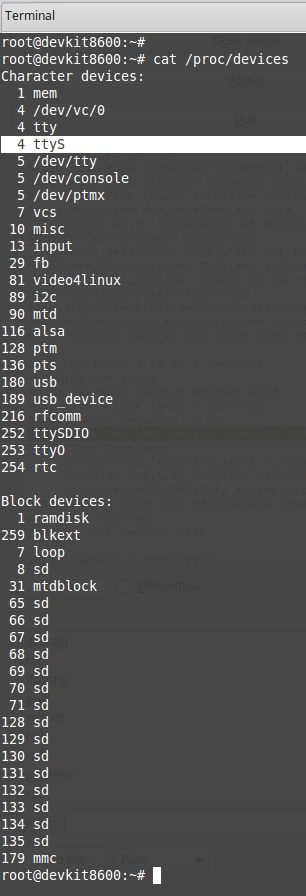
\includegraphics[width=0.42\textwidth]{341.jpg}
\caption{Mise en évidence du port série dans /proc/devices}
\end{figure}

\begin{figure}[!]
\centering
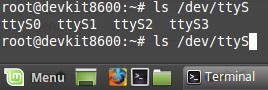
\includegraphics[width=0.3\textwidth]{342.jpg}
\caption{Mise en évidence du port série dans /dev}
\end{figure}

Le numéro en début de ligne dans le fichier /proc/devices correspond au numéro mineur, qui indique si les périphériques sont gérés par le même driver.

\newpage

\subsection{Question 3.5}

Voici une rapide description des dossiers :

\begin{figure}[h]
\centering
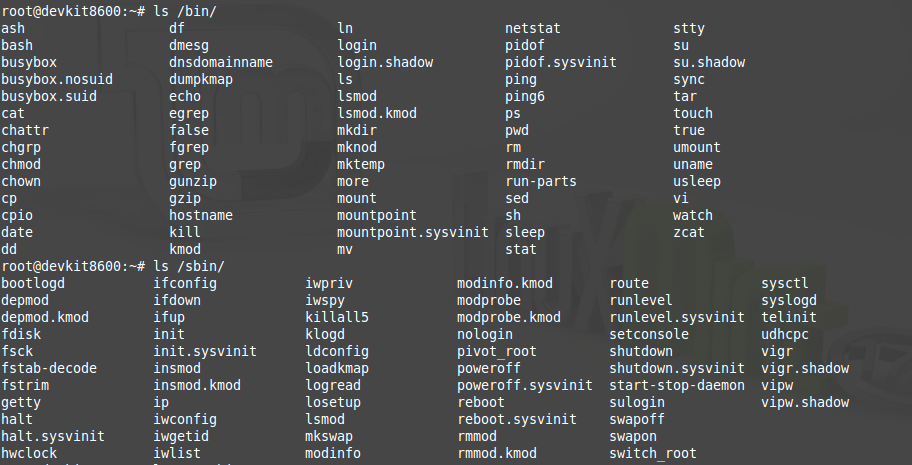
\includegraphics[width=0.8\textwidth]{screenstp5/35_bin_sbin.PNG}
\caption{Dossiers /bin et /sbin}
\end{figure}

\begin{itemize}
\item /bin : contient les binaires utilisables dès le boot, avant que la partition /usr soit montée. On y voit les commandes de base de type ls ou cat.
\item /sbin : même chose que /bin, mais commandes nécessitant des droits particuliers (superuser d'où le s)

\newpage
\begin{figure}[h]
\centering
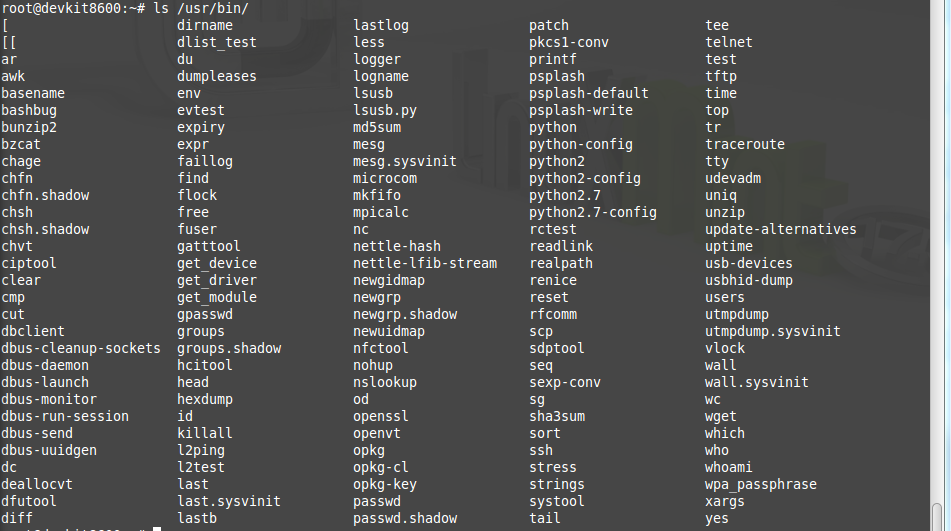
\includegraphics[width=0.8\textwidth]{screenstp5/35_usr_bin.PNG}
\caption{Dossier /usr/bin}
\end{figure}

\item /usr/bin : contient les binaires généraux du système (comme les applications que l'utilisateur installe)

\begin{figure}[h]
\centering
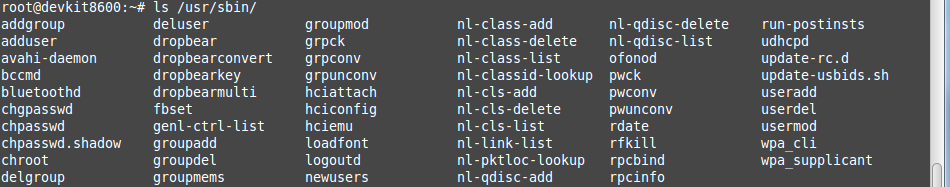
\includegraphics[width=0.8\textwidth]{screenstp5/35_usr_sbin.PNG}
\caption{Dossier /usr/sbin}
\end{figure}

\item /usr/sbin : même chose que /usr/bin, mais nécessitant des droits particuliers (superuser d'où le s)
\end{itemize}


\newpage

\section{Exercice 4 : Ajout de paquets}
\subsection{Question 4.1}

\begin{figure}[h]
	\centering
		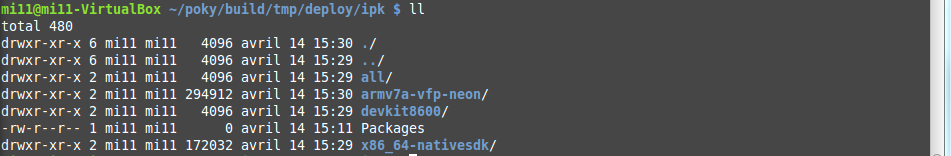
\includegraphics[width=1\textwidth]{41dossier_deploy_ipk.png}
		\caption{Dossier \textit{ipk}}
\end{figure}

Le dossier \textit{/home/mi11/poky/build/tmp/deploy/ipk} est organisé par architectures (x86/x64, devkit8600, armv7a, etc.).

\newpage

\begin{figure}[h]
	\centering
		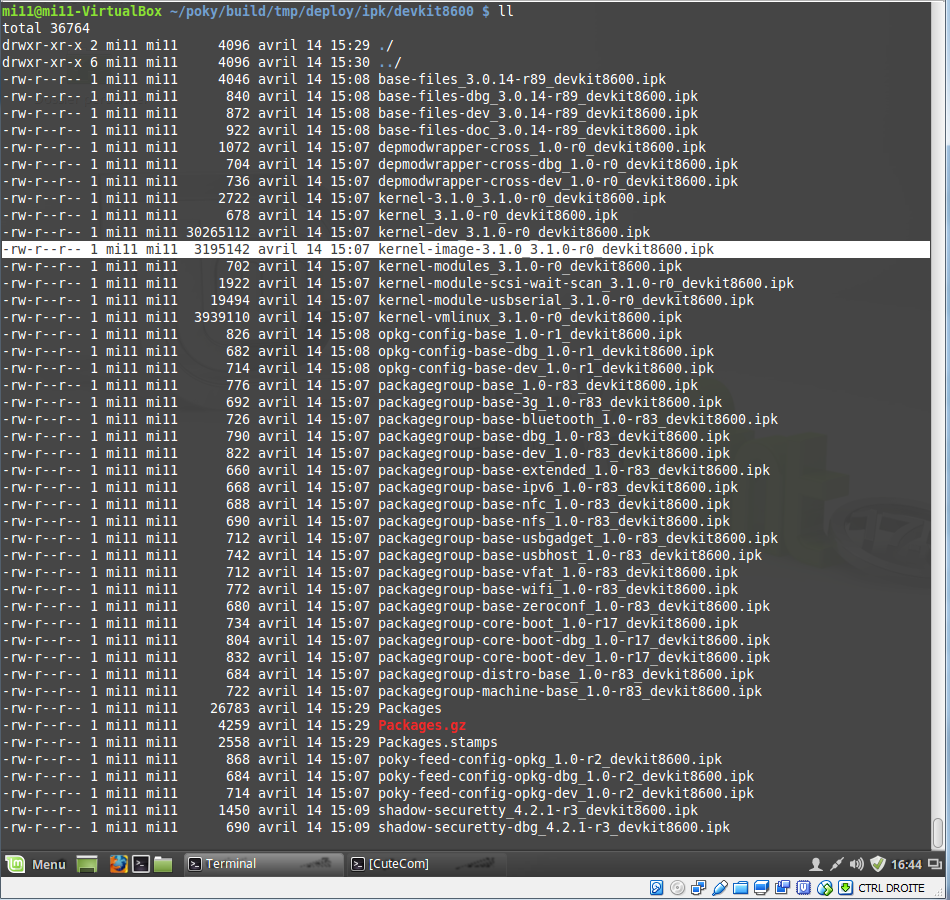
\includegraphics[width=1\textwidth]{41ou_se_trouve_le_noyau.png}
		\caption{Dossier \textit{ipk/devkit800}}
\end{figure}

Les sous-dossiers contiennent des paquets d'extension \textit{.ipk}. Le noyau se trouve dans le sous-dossier \textit{devkit8600} comme nous pouvons le voir sur la copie d'écran ci-dessus. Quant au paquet \textit{libxml2}, il se trouve dans le sous-dossier \textit{armv7a-vfp-neon}.

\newpage

\subsection{Question 4.2}

Les différents paquets relatifs à \textit{libxml2} sont visibles sur la copie d'écran suivante.

\begin{figure}[h]
	\centering
		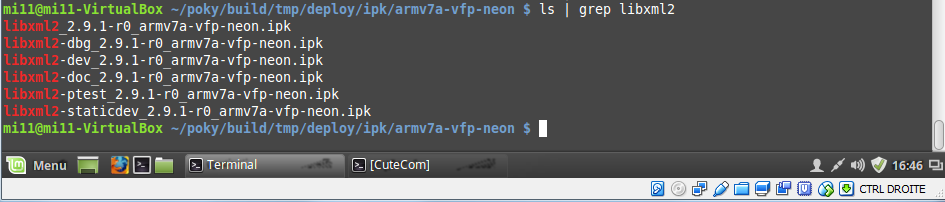
\includegraphics[width=1\textwidth]{42.png}
		\caption{Dossier \textit{ipk/armv7a-vfp-neon}}
\end{figure}

Nous avons ensuite copié le fichier 
\begin{verbatim}
libxml2_2.9.1-r0_armv7a-vfp-neon.ipk 
\end{verbatim}
dans le système de fichiers de la cible et nous avons installé le paquet avec la commande suivante : 
\begin{verbatim}
opkg install libxml2_2.9.1-r0_armv7a-vfp-neon.ipk
\end{verbatim}


\subsection{Question 4.3}

La première méthode pour copier le fichier dans le système de fichiers de la cible consiste à utiliser directement la commande \textit{cp} comme suit : 
\begin{verbatim}
sudo cp libxml2_2.9.1-r0_armv7a-vfp-neon.ipk /tftpboot/rootfs/home/root/
\end{verbatim}

La deuxième méthode consiste à copier le fichier à distance via la commande \textit{scp} qui se base sur \textit{ssh} comme suit : 
\begin{verbatim}
scp libxml2_2.9.1-r0_armv7a-vfp-neon.ipk root@192.168.1.6:/home/root/
\end{verbatim}

\subsection{Question 4.4}

Les fichiers de \textit{libxml2} installés par le gestionnaire de paquets se trouvent dans le dossier \textit{/usr/lib} de notre cible.

\begin{figure}[h]
	\centering
		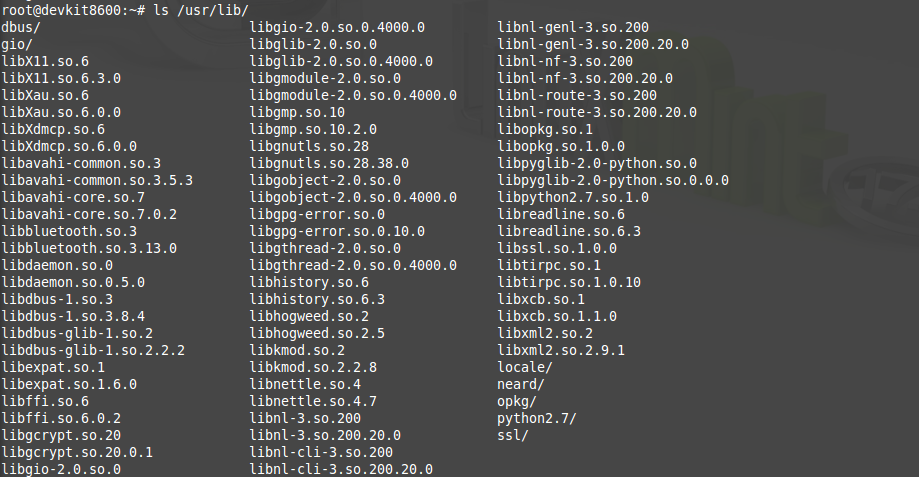
\includegraphics[width=1\textwidth]{44.png}
		\caption{Dossier \textit{/usr/lib}}
\end{figure}

Ce dossier contient des fichiers \textit{shared object} (.so) qui sont des librairies/bibliothèques partagées dynamiques.
Les .so sont des bibliothèques qui se chargent en mémoire au moment de l'exécution d'un programme qui les utilisent. Si plusieurs programmes les utilisant sont lancés en même temps, une seule instance de la bibliothèque dynamique réside en mémoire.
\newpage

\section{Exercice 5 : Compilation manuelle du noyau}
\subsection{Question 5.1}

La page 72 de la documentation nous dit qu'il est possible d'allumer et d'éteindre les LEDs via les commandes suivantes :
\begin{verbatim}
root@DevKit8600:~# echo 1 > /sys/class/leds/user_led/brightness
root@DevKit8600:~# echo 0 > /sys/class/leds/user_led/brightness
\end{verbatim}

Comme le dossier 
\begin{verbatim} 
user_led 
\end{verbatim} 
n'existe pas ce n'est pas opérationnel.

\subsection{Question 5.2}

Nous avons ensuite compiler manuellement le noyau via la chaîne de compilation croisée en exécutant le script suivant :
\begin{verbatim} 
source /opt/poky/1.7.3/environment-setup-armv7a-vfp-neon-poky-linux-gnueabi
unset LDFLAGS
\end{verbatim} 

Le fichier ci-dessus sert à mettre en place l'environnement de compilation de manière à avoir les bons préfixes pour une compilation croisée.
Le préfixe de la chaîne de compilation croisée est \textit{arm-poky-linux-gnueabi-}.

\subsection{Question 5.3}

Pour obtenir la liste des configurations par défaut du noyau pour une architecture ARM, il faut utiliser la commande \textit{make ARCH=arm help}.
Les configurations par défaut possibles pour la carte \textit{devkit8600} sont visibles sur la copie d'écran ci-dessous :

\begin{figure}[h]
	\centering
		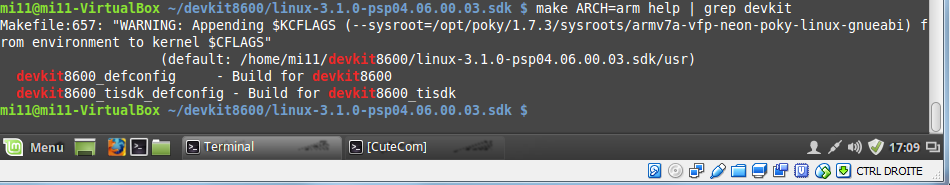
\includegraphics[width=1\textwidth]{53.png}
		\caption{Configurations par défaut de \textit{devkit8600}}
\end{figure}

Nous avons retenu uniquement la première configuration et nous l'avons mise en place via la commande suivante : 
\begin{verbatim} 
make devkit8600_defconfig
\end{verbatim} 

\subsection{Question 5.4}

Ensuite, nous avons lancé la personnalisation du noyau via la commande suivante : \textit{make ARCH=arm menuconfig}.
Le but étant d'ajouter un driver pour les LEDs connectées par GPIO.
Pour cela, nous avons activé l'option \textit{LED Support for GPIO connected LEDs} comme on peut le voir sur la copie d'écran suivante.

\newpage
\begin{figure}[h]
	\centering
		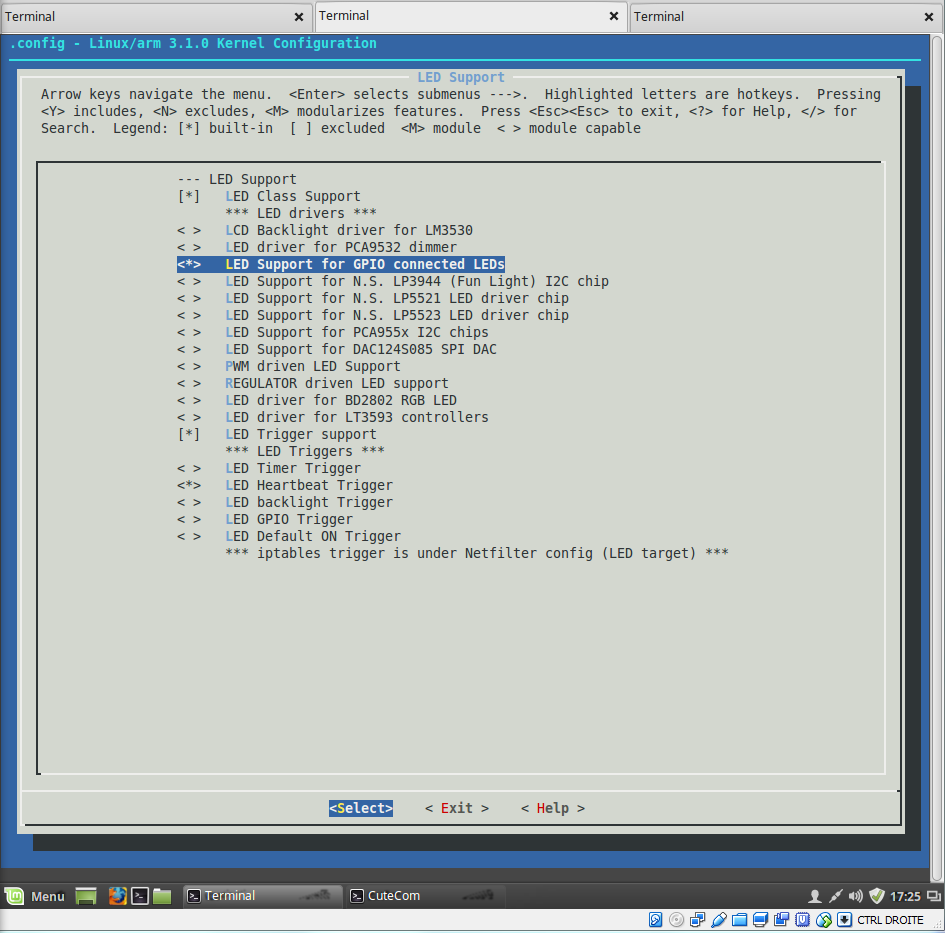
\includegraphics[width=1\textwidth]{54.png}
		\caption{Activation du driver pour les LEDs}
\end{figure}

\newpage

Ce driver peut être activé via deux modes, \textit{modularizes features} ou \textit{built-in}. Le premier mode est utilisé si l'on souhaite ajouter un driver en tant que module qui sera chargé en mémoire uniquement en cas de besoin et déchargé lorsque le kernel n'en a pas plus besoin. Ceci est utile lorsque l'on souhaite avoir un kernel pas très lourd.
Quant au deuxième mode, le driver sera directement intégré au kernel et il sera disponible tout le temps. Le kernel sera donc plus gros, plus lent et utilisera plus de mémoire.
Dans notre cas, nous avons utilisé le mode \textit{built-in}.\newline

Nous avons ensuite compiler notre noyau avec la commande suivante : \textit{make ARCH=arm uImage -j2}.

\subsection{Question 5.5}

Le résultat de la compilation se trouve dans \textit{arch/arm/boot/uImage}.

Nous avons ensuite copier le fichier uImage dans /tftpboot pour qu'il soit utilisé par la cible puis nous l'avons démarré.

\newpage

\subsection{Question 5.6}

Pour vérifier dans les logs de démarrage que le noyau utilisé est bien celui qui vient d'être compilé, il suffit de lire la date de compilation :

\begin{figure}[h]
	\centering
		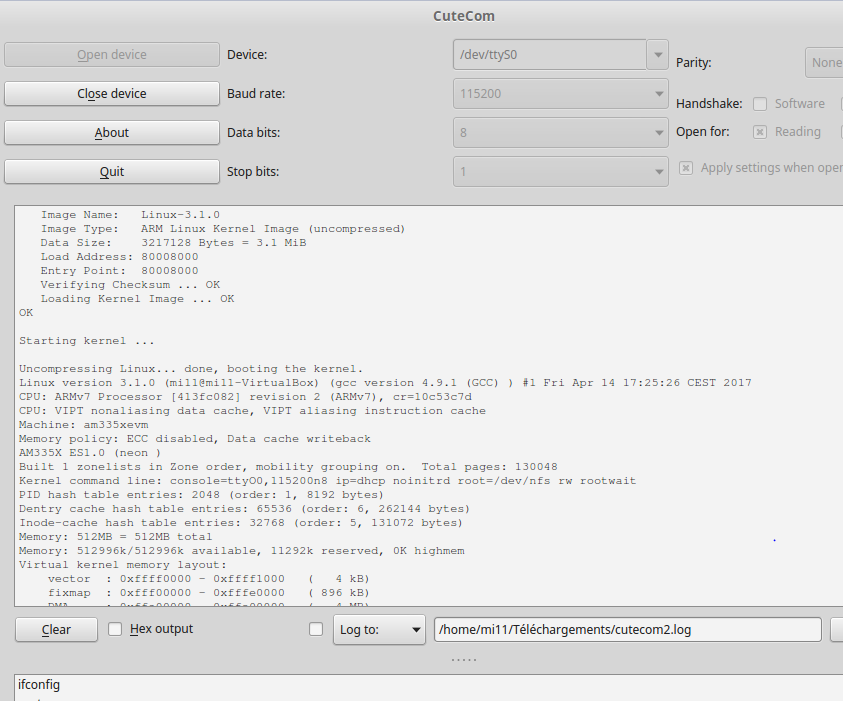
\includegraphics[width=1\textwidth]{56.png}
		\caption{Logs de démarrage}
\end{figure}

Nous pouvons lire sur la copie d'écran précédente la ligne suivante : 
\begin{verbatim}
Linux version 3.1.0 (mi11@mi11-VirtualBox) (gcc version 4.9.1 (GCC) ) 
#1 Fri Apr 14 17:25:26 CEST 2017
\end{verbatim}

La date de compilation du noyau correspond bien à celui qui vient d'être compilé.



\subsection{Question 5.7}

Pour vérifier dans les logs de démarrage que la fonctionnalité ajoutée est bien présente, on peut utiliser la commande \textit{dmesg} pour afficher les messages du kernel :

\begin{figure}[h]
	\centering
		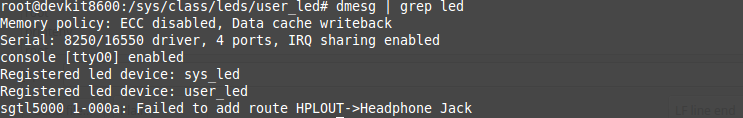
\includegraphics[width=1\textwidth]{57.png}
		\caption{Logs du kernel}
\end{figure}

Le driver a bien été ajouté et le dossier 
\begin{verbatim}
used_led 
\end{verbatim}
a été crée.



\appendix
\chapter{Messages de sortie du terminal entre l'allumage de la cible et le prompt de login}
\begin{lstlisting}[caption=Messages de sortie du terminal entre l'allumage de la cible et le prompt de login, label=message_sortie]
CCCCCCCC
U-Boot SPL 2011.09-svn (May 22 2012 - 11:19:00)
Texas Instruments Revision detection unimplemented
Booting from NAND...


U-Boot 2011.09-svn (May 22 2012 - 11:19:00)

I2C:   ready
DRAM:  512 MiB
WARNING: Caches not enabled
Did not find a recognized configuration, assuming General purpose EVM in Profile 0 with Daughter board
NAND:  HW ECC Hamming Code selected
512 MiB
MMC:   OMAP SD/MMC: 0
Net:   cpsw
Hit any key to stop autoboot:  3 \0x08\0x08\0x08 2 \0x08\0x08\0x08 1 \0x08\0x08\0x08 0 
Card did not respond to voltage select!
Booting from network ...
miiphy read id fail
link up on port 0, speed 100, full duplex
BOOTP broadcast 1
DHCP client bound to address 192.168.1.6
Using cpsw device
TFTP from server 192.168.1.1; our IP address is 192.168.1.6
Filename 'uImage'.
Load address: 0x82000000
Loading: *\0x08#################################################################
\0x09 #################################################################
\0x09 #################################################################
\0x09 #################################################################
\0x09 #################################################################
\0x09 #################################################################
\0x09 #################################################################
\0x09 #################################################################
\0x09 #################################################################
\0x09 ###########################################
done
Bytes transferred = 3215152 (310f30 hex)
## Booting kernel from Legacy Image at 82000000 ...
   Image Name:   Linux-3.1.0
   Image Type:   ARM Linux Kernel Image (uncompressed)
   Data Size:    3215088 Bytes = 3.1 MiB
   Load Address: 80008000
   Entry Point:  80008000
   Verifying Checksum ... OK
   Loading Kernel Image ... OK
OK

Starting kernel ...

Uncompressing Linux... done, booting the kernel.
Linux version 3.1.0 (mi11@mi11-VirtualBox) (gcc version 4.9.1 (GCC) ) #1 Mon Apr 10 18:15:11 CEST 2017
CPU: ARMv7 Processor [413fc082] revision 2 (ARMv7), cr=10c53c7d
CPU: VIPT nonaliasing data cache, VIPT aliasing instruction cache
Machine: am335xevm
Memory policy: ECC disabled, Data cache writeback
AM335X ES1.0 (neon )
Built 1 zonelists in Zone order, mobility grouping on.  Total pages: 130048
Kernel command line: console=ttyO0,115200n8 ip=dhcp noinitrd root=/dev/nfs rw rootwait
PID hash table entries: 2048 (order: 1, 8192 bytes)
Dentry cache hash table entries: 65536 (order: 6, 262144 bytes)
Inode-cache hash table entries: 32768 (order: 5, 131072 bytes)
Memory: 512MB = 512MB total
Memory: 512996k/512996k available, 11292k reserved, 0K highmem
Virtual kernel memory layout:
    vector  : 0xffff0000 - 0xffff1000   (   4 kB)
    fixmap  : 0xfff00000 - 0xfffe0000   ( 896 kB)
    DMA     : 0xffa00000 - 0xffe00000   (   4 MB)
    vmalloc : 0xe0800000 - 0xf8000000   ( 376 MB)
    lowmem  : 0xc0000000 - 0xe0000000   ( 512 MB)
    modules : 0xbf000000 - 0xc0000000   (  16 MB)
      .text : 0xc0008000 - 0xc05c6000   (5880 kB)
      .init : 0xc05c6000 - 0xc05ff000   ( 228 kB)
      .data : 0xc0600000 - 0xc065e618   ( 378 kB)
       .bss : 0xc065e63c - 0xc0699694   ( 237 kB)
NR_IRQS:396
IRQ: Found an INTC at 0xfa200000 (revision 5.0) with 128 interrupts
Total of 128 interrupts on 1 active controller
OMAP clockevent source: GPTIMER1 at 25000000 Hz
OMAP clocksource: GPTIMER2 at 25000000 Hz
sched_clock: 32 bits at 25MHz, resolution 40ns, wraps every 171798ms
Console: colour dummy device 80x30
Calibrating delay loop... 718.02 BogoMIPS (lpj=3590144)
pid_max: default: 32768 minimum: 301
Security Framework initialized
Mount-cache hash table entries: 512
CPU: Testing write buffer coherency: ok
devtmpfs: initialized
print_constraints: dummy: 
NET: Registered protocol family 16
GPMC revision 6.0
OMAP GPIO hardware version 0.1
omap_l3_smx omap_l3_smx.0: couldn't find resource
omap_mux_init: Add partition: #1: core, flags: 0
 omap_i2c.1: alias fck already exists
The board is general purpose EVM in profile 0
 omap_hsmmc.0: alias fck already exists
 omap_hsmmc.2: alias fck already exists
Configure Bluetooth Enable pin...
error setting wl12xx data
 omap2_mcspi.1: alias fck already exists
 omap2_mcspi.2: alias fck already exists
bio: create slab <bio-0> at 0
SCSI subsystem initialized
usbcore: registered new interface driver usbfs
usbcore: registered new interface driver hub
usbcore: registered new device driver usb
registerd cppi-dma Intr @ IRQ 17
Cppi41 Init Done Qmgr-base(e083a000) dma-base(e0838000)
Cppi41 Init Done
omap_i2c omap_i2c.1: bus 1 rev4.0 at 100 kHz
Advanced Linux Sound Architecture Driver Version 1.0.24.
Bluetooth: Core ver 2.16
NET: Registered protocol family 31
Bluetooth: HCI device and connection manager initialized
Bluetooth: HCI socket layer initialized
Bluetooth: L2CAP socket layer initialized
Bluetooth: SCO socket layer initialized
Switching to clocksource gp timer
Switched to NOHz mode on CPU #0
musb-hdrc: version 6.0, ?dma?, otg (peripheral+host)
musb-hdrc musb-hdrc.0: dma type: dma-cppi41
musb-hdrc musb-hdrc.0: USB OTG mode controller at e080a000 using DMA, IRQ 18
musb-hdrc musb-hdrc.1: dma type: dma-cppi41
musb-hdrc musb-hdrc.1: USB OTG mode controller at e080c800 using DMA, IRQ 19
NET: Registered protocol family 2
IP route cache hash table entries: 4096 (order: 2, 16384 bytes)
TCP established hash table entries: 16384 (order: 5, 131072 bytes)
TCP bind hash table entries: 16384 (order: 4, 65536 bytes)
TCP: Hash tables configured (established 16384 bind 16384)
TCP reno registered
UDP hash table entries: 256 (order: 0, 4096 bytes)
UDP-Lite hash table entries: 256 (order: 0, 4096 bytes)
NET: Registered protocol family 1
RPC: Registered named UNIX socket transport module.
RPC: Registered udp transport module.
RPC: Registered tcp transport module.
RPC: Registered tcp NFSv4.1 backchannel transport module.
NetWinder Floating Point Emulator V0.97 (double precision)
VFS: Disk quotas dquot_6.5.2
Dquot-cache hash table entries: 1024 (order 0, 4096 bytes)
JFFS2 version 2.2. (NAND) (SUMMARY)  \0xc2\0xa9 2001-2006 Red Hat, Inc.
msgmni has been set to 1001
io scheduler noop registered
io scheduler deadline registered
io scheduler cfq registered (default)
Could not set LED4 to fully on
da8xx_lcdc da8xx_lcdc.0: GLCD: Found AT043TN24 panel
Console: switching to colour frame buffer device 60x34
Serial: 8250/16550 driver, 4 ports, IRQ sharing enabled
omap_uart.0: ttyO0 at MMIO 0x44e09000 (irq = 72) is a OMAP UART0
console [ttyO0] enabled
omap_uart.1: ttyO1 at MMIO 0x48022000 (irq = 73) is a OMAP UART1
omap_uart.2: ttyO2 at MMIO 0x48024000 (irq = 74) is a OMAP UART2
omap_uart.3: ttyO3 at MMIO 0x481a6000 (irq = 44) is a OMAP UART3
omap_uart.4: ttyO4 at MMIO 0x481a8000 (irq = 45) is a OMAP UART4
omap_uart.5: ttyO5 at MMIO 0x481aa000 (irq = 46) is a OMAP UART5
brd: module loaded
loop: module loaded
i2c-core: driver [tsl2550] using legacy suspend method
i2c-core: driver [tsl2550] using legacy resume method
mtdoops: mtd device (mtddev=name/number) must be supplied
omap2-nand driver initializing
ONFI flash detected
ONFI param page 0 valid
NAND device: Manufacturer ID: 0xad, Chip ID: 0xdc (Hynix H27U4G8F2DTR-BC)
Creating 8 MTD partitions on "omap2-nand.0":
0x000000000000-0x000000020000 : "SPL"
0x000000020000-0x000000040000 : "SPL.backup1"
0x000000040000-0x000000060000 : "SPL.backup2"
0x000000060000-0x000000080000 : "SPL.backup3"
0x000000080000-0x000000260000 : "U-Boot"
0x000000260000-0x000000280000 : "U-Boot Env"
0x000000280000-0x000000780000 : "Kernel"
0x000000780000-0x000020000000 : "File System"
OneNAND driver initializing
davinci_mdio davinci_mdio.0: davinci mdio revision 1.6
davinci_mdio davinci_mdio.0: detected phy mask ffffffef
davinci_mdio.0: probed
davinci_mdio davinci_mdio.0: phy[4]: device 0:04, driver unknown
CAN device driver interface
CAN bus driver for Bosch D_CAN controller 1.0
d_can d_can: d_can device registered (irq=55, irq_obj=56)
usbcore: registered new interface driver cdc_ether
usbcore: registered new interface driver cdc_subset
Initializing USB Mass Storage driver...
usbcore: registered new interface driver usb-storage
USB Mass Storage support registered.
 gadget: using random self ethernet address
 gadget: using random host ethernet address
usb0: MAC 06:50:55:8c:0c:93
usb0: HOST MAC 62:9a:93:a2:1e:53
 gadget: Ethernet Gadget, version: Memorial Day 2008
 gadget: g_ether ready
musb-hdrc musb-hdrc.0: MUSB HDRC host driver
musb-hdrc musb-hdrc.0: new USB bus registered, assigned bus number 1
usb usb1: New USB device found, idVendor=1d6b, idProduct=0002
usb usb1: New USB device strings: Mfr=3, Product=2, SerialNumber=1
usb usb1: Product: MUSB HDRC host driver
usb usb1: Manufacturer: Linux 3.1.0 musb-hcd
usb usb1: SerialNumber: musb-hdrc.0
hub 1-0:1.0: USB hub found
hub 1-0:1.0: 1 port detected
musb-hdrc musb-hdrc.1: MUSB HDRC host driver
musb-hdrc musb-hdrc.1: new USB bus registered, assigned bus number 2
usb usb2: New USB device found, idVendor=1d6b, idProduct=0002
usb usb2: New USB device strings: Mfr=3, Product=2, SerialNumber=1
usb usb2: Product: MUSB HDRC host driver
usb usb2: Manufacturer: Linux 3.1.0 musb-hcd
usb usb2: SerialNumber: musb-hdrc.1
hub 2-0:1.0: USB hub found
hub 2-0:1.0: 1 port detected
mousedev: PS/2 mouse device common for all mice
input: ti-tsc-adcc as /devices/platform/tsc/input/input0
omap_rtc omap_rtc: rtc core: registered omap_rtc as rtc0
i2c /dev entries driver
Linux video capture interface: v2.00
usbcore: registered new interface driver uvcvideo
USB Video Class driver (1.1.1)
OMAP Watchdog Timer Rev 0x01: initial timeout 60 sec
Bluetooth: HCI UART driver ver 2.2
Bluetooth: HCI H4 protocol initialized
Bluetooth: HCI BCSP protocol initialized
Bluetooth: HCILL protocol initialized
Bluetooth: HCIATH3K protocol initialized
cpuidle: using governor ladder
cpuidle: using governor menu
usbcore: registered new interface driver usbhid
usbhid: USB HID core driver
usbcore: registered new interface driver snd-usb-audio
_regulator_get: 1-000a supply VDDA not found, using dummy regulator
_regulator_get: 1-000a supply VDDIO not found, using dummy regulator
_regulator_get: 1-000a supply VDDD not found, using dummy regulator
sgtl5000 1-000a: sgtl5000 revision 17
print_constraints: 1-000a: 850 <--> 1600 mV at 1200 mV normal 
_regulator_get: 1-000a supply VDDA not found, using dummy regulator
_regulator_get: 1-000a supply VDDIO not found, using dummy regulator
sgtl5000 1-000a: Using internal LDO instead of VDDD
mmc1: card claims to support voltages below the defined range. These will be ignored.
sgtl5000 1-000a: Failed to add route HPLOUT->Headphone Jack
sgtl5000 1-000a: dapm: unknown pin MONO_LOUT
sgtl5000 1-000a: dapm: unknown pin HPLCOM
sgtl5000 1-000a: dapm: unknown pin HPRCOM
asoc: sgtl5000 <-> davinci-mcasp.0 mapping ok
ALSA device list:
  #0: AM335X EVM
oprofile: hardware counters not available
oprofile: using timer interrupt.
nf_conntrack version 0.5.0 (8015 buckets, 32060 max)
ip_tables: (C) 2000-2006 Netfilter Core Team
TCP cubic registered
NET: Registered protocol family 17
can: controller area network core (rev 20090105 abi 8)
NET: Registered protocol family 29
can: raw protocol (rev 20090105)
can: broadcast manager protocol (rev 20090105 t)
Bluetooth: RFCOMM TTY layer initialized
Bluetooth: RFCOMM socket layer initialized
Bluetooth: RFCOMM ver 1.11
Bluetooth: BNEP (Ethernet Emulation) ver 1.3
Bluetooth: BNEP filters: protocol multicast
Bluetooth: HIDP (Human Interface Emulation) ver 1.2
Registering the dns_resolver key type
VFP support v0.3: implementor 41 architecture 3 part 30 variant c rev 3
ThumbEE CPU extension supported.
_regulator_get: mpu.0 supply mpu not found, using dummy regulator
omap2_set_init_voltage: Fail set voltage-dpll_mpu_ck(f=720000000 v=1260000)on vddmpu
omap2_set_init_voltage: unable to set vdd_mpu
Detected MACID=0:18:30:fe:7b:f6
input: gpio-keys as /devices/platform/gpio-keys/input/input1
omap_rtc omap_rtc: setting system clock to 2000-01-01 00:00:00 UTC (946684800)
mmc1: queuing unknown CIS tuple 0x91 (3 bytes)

CPSW phy found : id is : 0x4dd072
PHY 0:01 not found
mmc1: new SDIO card at address 0001
PHY: 0:04 - Link is Up - 100/Full
Sending DHCP requests ., OK
IP-Config: Got DHCP answer from 192.168.1.1, my address is 192.168.1.6
IP-Config: Complete:
     device=eth0, addr=192.168.1.6, mask=255.255.255.0, gw=255.255.255.255,
     host=192.168.1.6, domain=, nis-domain=(none),
     bootserver=192.168.1.1, rootserver=192.168.1.1, rootpath=/tftpboot/rootfs
VFS: Mounted root (nfs filesystem) on device 0:15.
devtmpfs: mounted
Freeing init memory: 228K

INIT: version 2.88 booting

Starting udev
udevd[718]: starting version 182
bootlogd: cannot allocate pseudo tty: No such file or directory
Populating dev cache
Fri Apr 14 13:12:58 UTC 2017

INIT: Entering runlevel: 5

Configuring network interfaces... ifup skipped for nfsroot interface eth0
run-parts: /etc/network/if-pre-up.d/nfsroot exited with code 1
Starting system message bus: dbus.
Starting Dropbear SSH server: Generating key, this may take a while...
Public key portion is:
ssh-rsa AAAAB3NzaC1yc2EAAAADAQABAAABAQDHQW67zEKPRIeKx6VZxLER0R/2HThSN/SWD3fMk23eXy9j3PudyVMJfjGBF258qnZNicoMsK0Mx5JrpV124XKCzvKTAYsMjLc67WdqcX73zSzt1Cplk99ATrT3SKK+Dq16Nld2ZuhfGDidLPvrSqOfRaUYRH6048XV/E7penoQ8oP2tJV0kiGnXRQMoqSyLyZFWW/0xNzatB/Wr6o+I7Iboc2KWDyOu8caJxP4fxrV/4zEjyTvSQCBCzwuv2RSFPJV7lleMD2XkKN+QOGCgG1Eq8TgrNDU0Jps+RelENrtkj+lgVJF2odabmPMtmsB+8lhtgdgk8wth0dbjQzedRFt root@devkit8600
Fingerprint: md5 a7:0c:a2:b1:07:9a:77:98:01:7e:31:13:10:02:42:2c
dropbear.
Starting rpcbind daemon...rpcbind: cannot create socket for udp6

rpcbind: cannot create socket for tcp6

done.
Starting syslogd/klogd: done
 * Starting Avahi mDNS/DNS-SD Daemon: avahi-daemon
   ...done.
Starting Telephony daemon
Starting Linux NFC daemon
/etc/rc5.d/S64neard: line 26: /usr/lib/neard/nfc/neard: No such file or directory


Poky (Yocto Project Reference Distro) 1.7.3 devkit8600 /dev/ttyO0



devkit8600 login: root
root@devkit8600:~# 
\end{lstlisting}



\end{document}

